\documentclass[a4paper,twoside]{article}

\usepackage{epsfig}
\usepackage{subfigure}
\usepackage{calc}
\usepackage{amssymb}
\usepackage{amstext}
\usepackage{amsmath}
\usepackage{amsthm}
\usepackage{multicol}
\usepackage{pslatex}
\usepackage{apalike}
\usepackage{SCITEPRESS}
\usepackage{mhchem}
\usepackage{latexsym}
\usepackage{algorithm2e}
\usepackage[noend]{algpseudocode}
\usepackage{subfig}
\usepackage{graphicx}
\makeatletter
\def\BState{\State\hskip-\ALG@thistlm}
\makeatother


% Please add other packages that you may need BEFORE the SCITEPRESS.sty package.

\subfigtopskip=0pt
\subfigcapskip=0pt
\subfigbottomskip=0pt

\begin{document}

\title{Easy Grader: An automatic exam grading tool based on conventional line detection algorithm}

\author{\authorname{Yang Xu, Lei Jiao}
\affiliation{Technical University of Berlin, Berlin, Germany}
\email{kabiyangvanx912@gmail.com, noahinde2014@gmail.com}
}


\keywords{Exam, Automatic grading, Hough Line Transform, cross detection, check mark detection}

\abstract{Grading massive amount of exam sheets is a burdensome work for graders even when the majority of the questions in the exam are multiple choice question. Since the answers of those questions are generally well structured, e.g. they are represented as check marks in a table, such a heavy job can finished by using a fully or semi-automatic grading program. In this paper we introduce a lightweight yet powerful tool that is implemented for this purpose based on some conventional methods and algorithms. In our experimental evaluation our implemented tool achieves a quite good performance on the collected data set with an overall accuracy rate 0.970 while the required time for processing each answer sheet takes less than $0.2s$ in most cases.}

\onecolumn \maketitle \normalsize \vfill

\section{\uppercase{Introduction}}
\label{sec:introduction}

\noindent At the beginning or the end of each semester the tutors in the department Computer Vision and Remote Sensing of Technical University of Berlin are always occupied with grading the final exam of Automatic Image Analysis or other courses for over 100 students. This work is considerably onerous even the the majority of the questions in the exam are multiple choice question. Figure \ref{fig:example_answer_sheet} is a example answer sheet taken from our created data set. As you can see here, the answers are represented as check marks(in our case they are crosses) and are placed within the table. The well structured check marks make it possible that grading the large amount of answer sheet automatically. Except for those crosses, it can be noticed that some of the rows are crossed out(e.g. the row corresponding to question 4 in figure \ref{fig:example_answer_sheet}) and the corresponding correct answers are allowed to be written in the non-occupied rows in the bottom of the table. Moreover, it is also very common correcting the a answer by covering the cross with a bunch of casually drafted curves(e.g. the cell in the row corresponding to question 2 and second column), which is named “self-corrected answer”. Those self-corrected answers obviously can not be treated as crosses anymore. The Objective of our project is to detect the all of aforementioned cases.\\
Detecting the cross can be approximately regard as the recognition of the handwritten character \textbf{X}, which inspires us to deploy handwritten characters recognition related techniques at first. During the last few decades the Recognition of offline images of handwritten characters has been widely studied \cite{arica2001overview} and recent studies on convolution neural networks(CNNs) have shown their power in image classification and segmentation. In recent years there have been lots of CNNs with various architectures proposed and it has been proven that most of them overperform  traditional methods. However, it can not be ignored that the success of applying CNN to image classification are based on the support of enormous labeled images.\\
In our cases, there are only in total 17 answer sheet available and in each of them the number of crosses are around 60. Such a small data set makes it impossible for us to implement an efficient CNN. Hence we tend to leverages the power of multiple classical algorithms in lines detection to solve the problem.\\
The remainder of the paper is structured as follows. Section 2 introduces theories that used in our implemented tool, while section 3 describes the essential ingredients for detecting cross or self-corrected answers including sheet preprocessing, table extraction etc. Section 4 shows the performance of the implemented tool on our created dataset with a conclusion being given in Section 5. 

\section{\uppercase{Theory}}
\subsection{Morphological Image Processing}
Due to the reason that the binary images are mostly produced by simple thresholding the images, which may cause the distortion by noise and textures. Morphological image processing is one of the approach to remove these noise and texture by accounting for the form and structure of the image. Morphological operations rely only on the relative ordering of pixel values, not on the numerical values.\\
Morphological techniques probe an image with small shape or template called a structuring element. It is useful to define some arbitrary neighborhood structures \cite{ravi2013morphological}.
\begin{figure}[!h]
  %\vspace{-0.2cm}
  \centering
  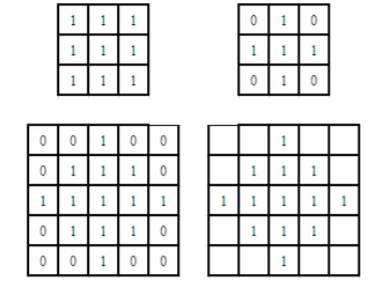
\includegraphics[width=0.8\columnwidth]{Latex/imgs/structelement.PNG}
  \caption{different types of structuring element}
  \label{fig:structelement}
 \end{figure}
In order to handle binary images, the morphological operation create the binary structuring element which is comprised by zeros and ones, and the ones can be defined as the neighborhood of the structuring element.
\subsubsection{Erosion and dilation}
The dilation operation makes an object to grow by size \cite{ravi2013morphological}. The dilation of an image A (set) by structuring element B is defined as
\begin{equation}
    \ce{A {$\oplus$} B} = \{ Z | \hat{(B)_{z}} \cap A\neq \emptyset \}
\end{equation}
If set B is reflected about its origin and shifted by z, then
the dilation of A by B is the set of all displacements z such that $\hat{B}$ and A have at least one common element. The dilation process enlarges the number of pixels with 1 and shrink the number of pixels with values 0. Moreover, the dilation process is mostly used to fill the holes in a continuous object.\\
Erosion, on the other hand, shrinks the size of the object. The Erosion process can be defined as
\begin{equation}
\ce{A {$\ominus$} B} = \{ Z | (B)_z \subseteq  A \}
\end{equation}
The erosion of image A by structuring element B is the set
of all points z such that the structuring element B is translated
by z is a subset of the image. After the operation the boundary pixels will be lost. The erosion process enlarges the number of pixels with 0 and shrinks the number of pixels with 1.
\subsubsection{Opening and closing}
The opening operation of an image A by a structuring element B is an erosion followed by a dilation, it can be denoted as
\begin{equation}
    A \circ B = (A \ce{$\ominus$} B)\ce{$\oplus$} B
\end{equation}
Opening can open up a gap between objects connected by narrow brige of pixels. Any regions reserved after erosion will be restored to their original size by dilation. The opening operation smoothes the outline of an object
clears the narrow bridges and also eliminates minor extensions
present in the object \cite{ravi2013morphological}.
The closing operation changes the order of occurrence of erosion and dilation operation, it can be defined as
\begin{equation}
    A \cdot B = (A \ce{$\oplus$} B)\ce{$\ominus$} B
\end{equation}
The closing operation though smoothes sections of contours
it in general blends narrow breaks and thin gaps. As a result it
eliminates small holes and fills gaps in the objects boundaries \cite{ravi2013morphological}.  
\subsection{Probabilistic Hough transform}
\label{sec:PHT}
The standard Hough transform \cite{duda1971use} is used to determine the parameters of features such as lines and curves within an image which each pixel represents part of an edge feature. The standard Hough transform map these pixels into polar coordinate system $(\rho, \theta)$ since each line can be written as:
\begin{equation}
    \rho = x\cos \theta + y\sin \theta
\end{equation}
\begin{equation}
    y = (-\dfrac{\cos \theta}{\sin \theta})x + \dfrac{\rho}{\sin \theta}
\end{equation}

Moreover, we can also define the family of lines that goes through a point $(x_0, y_0)$ as:
\begin{equation}
    \rho _{\theta} = x_0\cos \theta+y_0\sin \theta 
\end{equation}
so that each $(\rho_{\theta}, \theta)$ represents each line passes $(x_0, y_0)$. This is sometimes referred to as the voting stage. If multiple points in the image are collinear then their sinusoids in parameters space will cross. Thus, finding the points in parameter space where the most sinusoids cross gives the parameters for the lines in the input image. 
Probabilistic Hough transform proposed by Kiryati et al. \cite{kiryati1991probabilistic} is an optimization of Hough transform. It takes only a subset of points $m$ randomly from all the edge points $M$ and it is sufficient for line detection. The complexity of the voting stage can be reduced from $O(M,N_{\theta})$ to $O(m, N_{\theta})$. However, it is a trade-off between the accuracy and the speed of the algorithm, chossing a smaller value of $m$ will lead to a faster algorithm but the small features may no longer be detected. Moreover, Kiryati et al. performed an analysis of the effect of the threshold for the value of $m$, this threshold effect was confirmed with good results being obtained with as few as $2\%$ of edge points.

\section{\uppercase{Implementation}}
\subsection{System Overview}
\begin{figure}[!h]
  \centering
  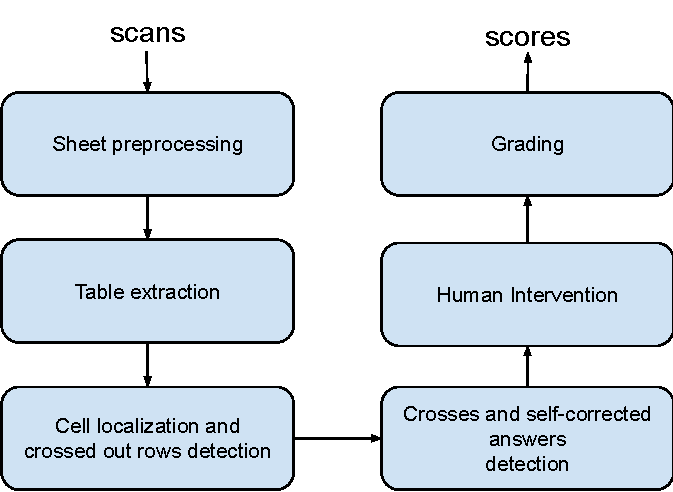
\includegraphics[width=\columnwidth]{Latex/imgs/SystemOverview.pdf}
  \caption{System diagram for grading the scanned answer sheets.}
  \label{fig:System_diagram}
 \end{figure}
Figure \ref{fig:System_diagram} shows the block diagram of our system for grading the scanned sheets. First, the scans will be prepossessed to generate the binary image. Then a couple of morphological operations will be applied to the binary image such that the characters, digits and even the crosses are been removed. The resulting in images only compose of horizontal and vertical lines. Based on those lines we can not only localize the cells but also can determine which rows of the tables have been crossed out and labels those rows. Then we will iterate over all cells from the extracted table and for each cell our proposed algorithm will be applied for detecting the cross and self-corrected answers. A well-designed algorithms or strategy is supposed to handle most of cases here. Since achieving an absolutely correct detection is extremely tough, it is necessary providing user the possibility to intervene and correct the results. Last, a simple scripts will be used for giving the corresponding grades by comparing the results and standard answers.   
 
 
\subsection{Preprocessing}
In this paper, the preprocessing part is made up of 
\begin{itemize}
    \item Read in image
    \item Remove noise
    \item Produce binary images
\end{itemize}
The steps above is succeeded with the help of OpenCV library, which is a convenient library to deal with images.
Gaussian blurring is the approach we used to remove noise. Gaussian blurring uses the normal distribution to give each neighboring pixel a weight. Therefore, the pixel value after the Gaussian blurring is the sum of all the pixels multiply with their weights in a $N\times N$ kernel. The blurring technique is widely used to remove noise.
After the Gaussian blurring, the images will be converted into binary images in order to detect contours.

\subsection{Table extraction}
Since the binary images are produced, the next step is to detect the location of the table. 
\begin{figure}[!h]
  %\vspace{-0.2cm}
  \centering
  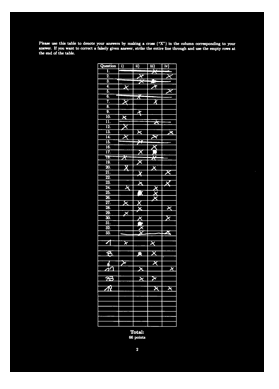
\includegraphics[width=\columnwidth]{Latex/imgs/binary.PNG}
  \caption{Binary image of the answer sheet}
  \label{fig:answersheet_binary}
 \end{figure}
Figure \ref{fig:answersheet_binary} is one of the answer sheet produced after preprocessing, In order to detect the table, the first step is to delete the characters and crosses and meanwhile preserve the lines of the table. The reason is that as described in the next section, it is necessary to get the coordinates of the pixels on the contours. If we directly detect the contours in such a binary image, we will get the contours of the characters and crosses, which can impose a challenge upon us for further localize cells. As mentioned in the theory part, the morphological opening operation is implemented. We created 2 kinds of structuring elements, one is a long but thin horizontal kernel with only 1 pixel wide, The other one is a long but thin vertical kernel. The morphological opening operation will first of all erode the characters in the answer sheet, then the dilation operation will return the remaining objects into its original size. After the morphological opening operation it remains only the long vertical lines and the long horizontal lines. \\
\begin{figure}[!h]
  %\vspace{-0.2cm}
  \centering
  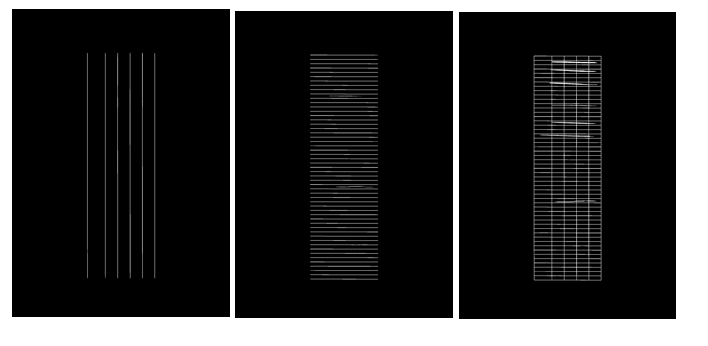
\includegraphics[width=\columnwidth]{Latex/imgs/addweight.PNG}
  \caption{add the images with vertical and horizontal lines }
  \label{fig:final table}
 \end{figure}
As shown in figure \ref{fig:final table}, the images that contain only vertical lines and only  horizontal lines will be added together and produce the final binary image of the table. Moreover, we can also find out that except for the horizontal or vertical lines, the lines used to cross out the specific rows of the table are retained in the resulting binary image, as depicted in the rightmost image of figure \ref{fig:final table}. It will be explained in the next section how to utilize those retrained lines to decide whether a row of the table is cross out or not. \\ 
 \begin{figure}[!h]
  \centering
  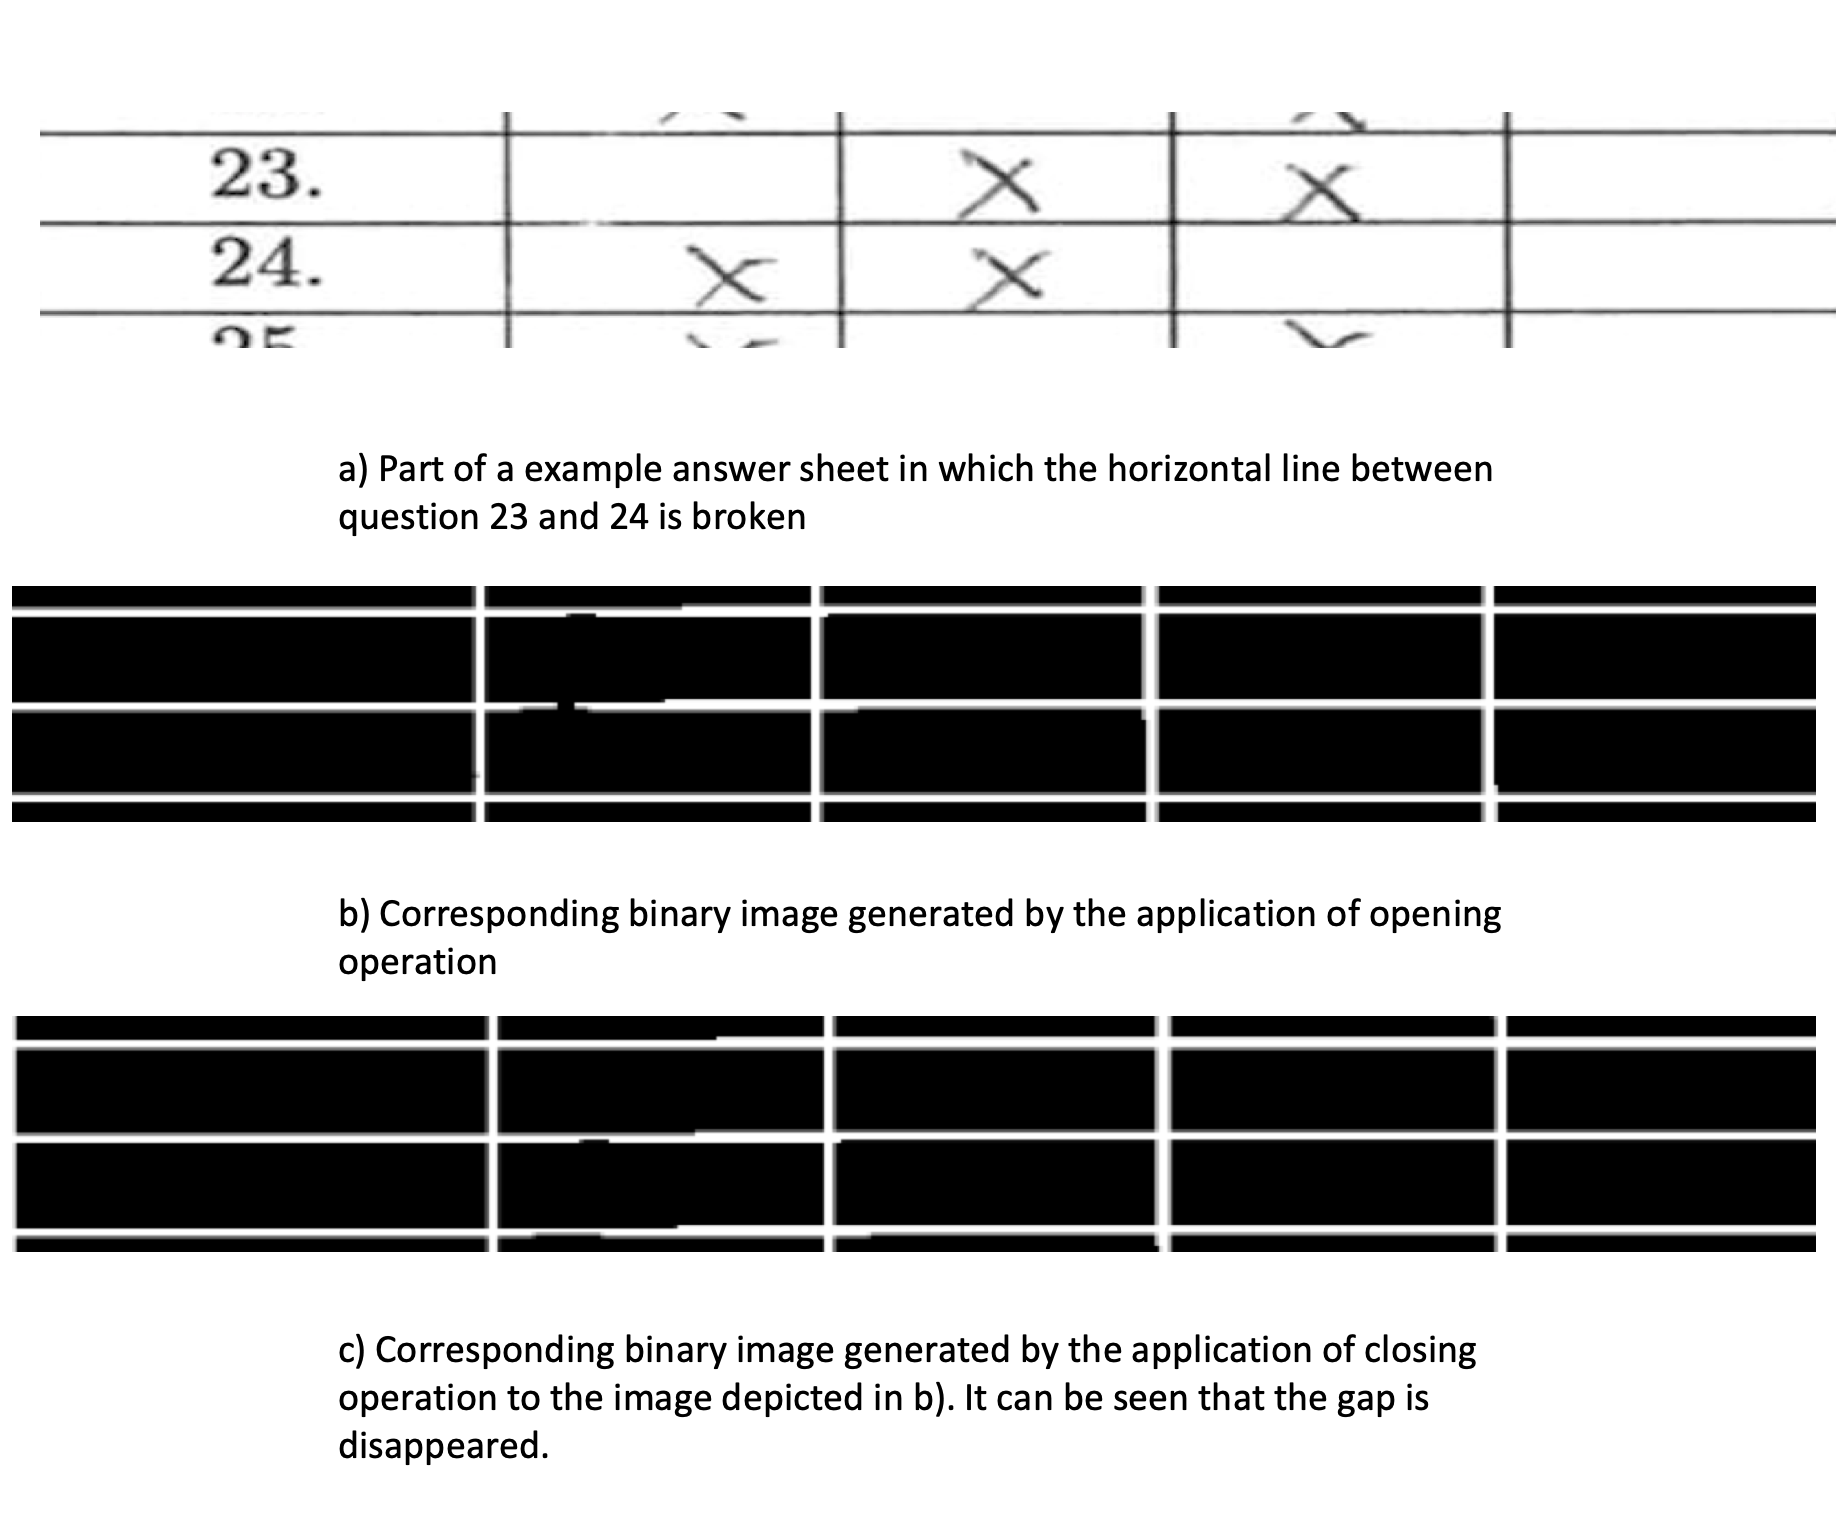
\includegraphics[width=\columnwidth]{Latex/imgs/sheet34.png}
  \caption{Line broken problem}
  \label{fig:sheet34}
 \end{figure}
The approach introduced in the next section for locating the cells are based on the detected contours of the cell, which means if the contours the cell is broken, then it will not able to be  regarded as a cell. In a few of scanned answer sheet, we have notice that a fraction of the horizontal lines of the the table are prone to be broken. For instance it is evident that there is a gap exising on the horizontal line between 23 and 24. As a result, both rows corresponding to question 23 and 24 will be treated as crossed out rows and accordingly the cross within these two rows can not be detected any more. A possible solution is applying the closing operation right after using the opening operations to the binary inverted image. As shown in Figure \ref{fig:sheet34}c) the gap can be perfectly eliminated.   

\subsection{Cell location determination and crossed out rows detection }
After the extraction of the table, the next step is to find out the location of each cell in the table. Moreover, although using the absolute location of the cell  is the easiest way to implement, e.g. using the value of width and the height of the cell as input parameter and calculate the position of the cells. It cannot be robust to different resolution. Therefore, we developed an algorithm to calculate the relative width and height between cells automatically with only a few thresholds as input parameters.
Firstly, by using the contours finder function on the binary image of the table, an array of all the detected boundaries will be returned. Afterwards, we approximate the rectangles in the array of contours, More specifically, by specifying the number of verticies as 4 and the maximum distance between the original curve and its approximation, this function can detect whether a contours is a closing polygon with 4 verticies and return the positions of the verticies. Then we will calculate the moments of the rectangles found in the last step. The calculated centroids are one of the most important input parameters to locate the positions of cells and to estimate which task and which answer a cell belongs to.\\
\begin{figure}[!h]
  %\vspace{-0.2cm}
  \centering
  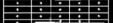
\includegraphics[width=0.5\columnwidth]{Latex/imgs/moments.PNG}
  \caption{the detected centroids of the cells}
  \label{fig:moments}
 \end{figure}
Next step is to estimate the height of the cells, Here we implemented K means to estimate the height of cells by input the heights of centroids in the frist and the second column and splite them into 2 clusters, the \textit{kmeans} function in OpenCV can return the centres of these 2 clusters, and the Euclidean distance between these centres is the result height of cells.
According to the observation of the answer sheet in fig \ref{fig:moments}, it can be found out a line is made up of 5 rectangles, i.e. 5 centroids. If we can find out the height of these 5 centroids are extremely close and the distance towards the last detected line is equal to the height of a cell, so these 5 centroids can be detected as a line. The final result of detected location of cell can be found in figure \ref{fig:locations of cells}
\begin{figure}[!h]
  %\vspace{-0.2cm}
  \centering
  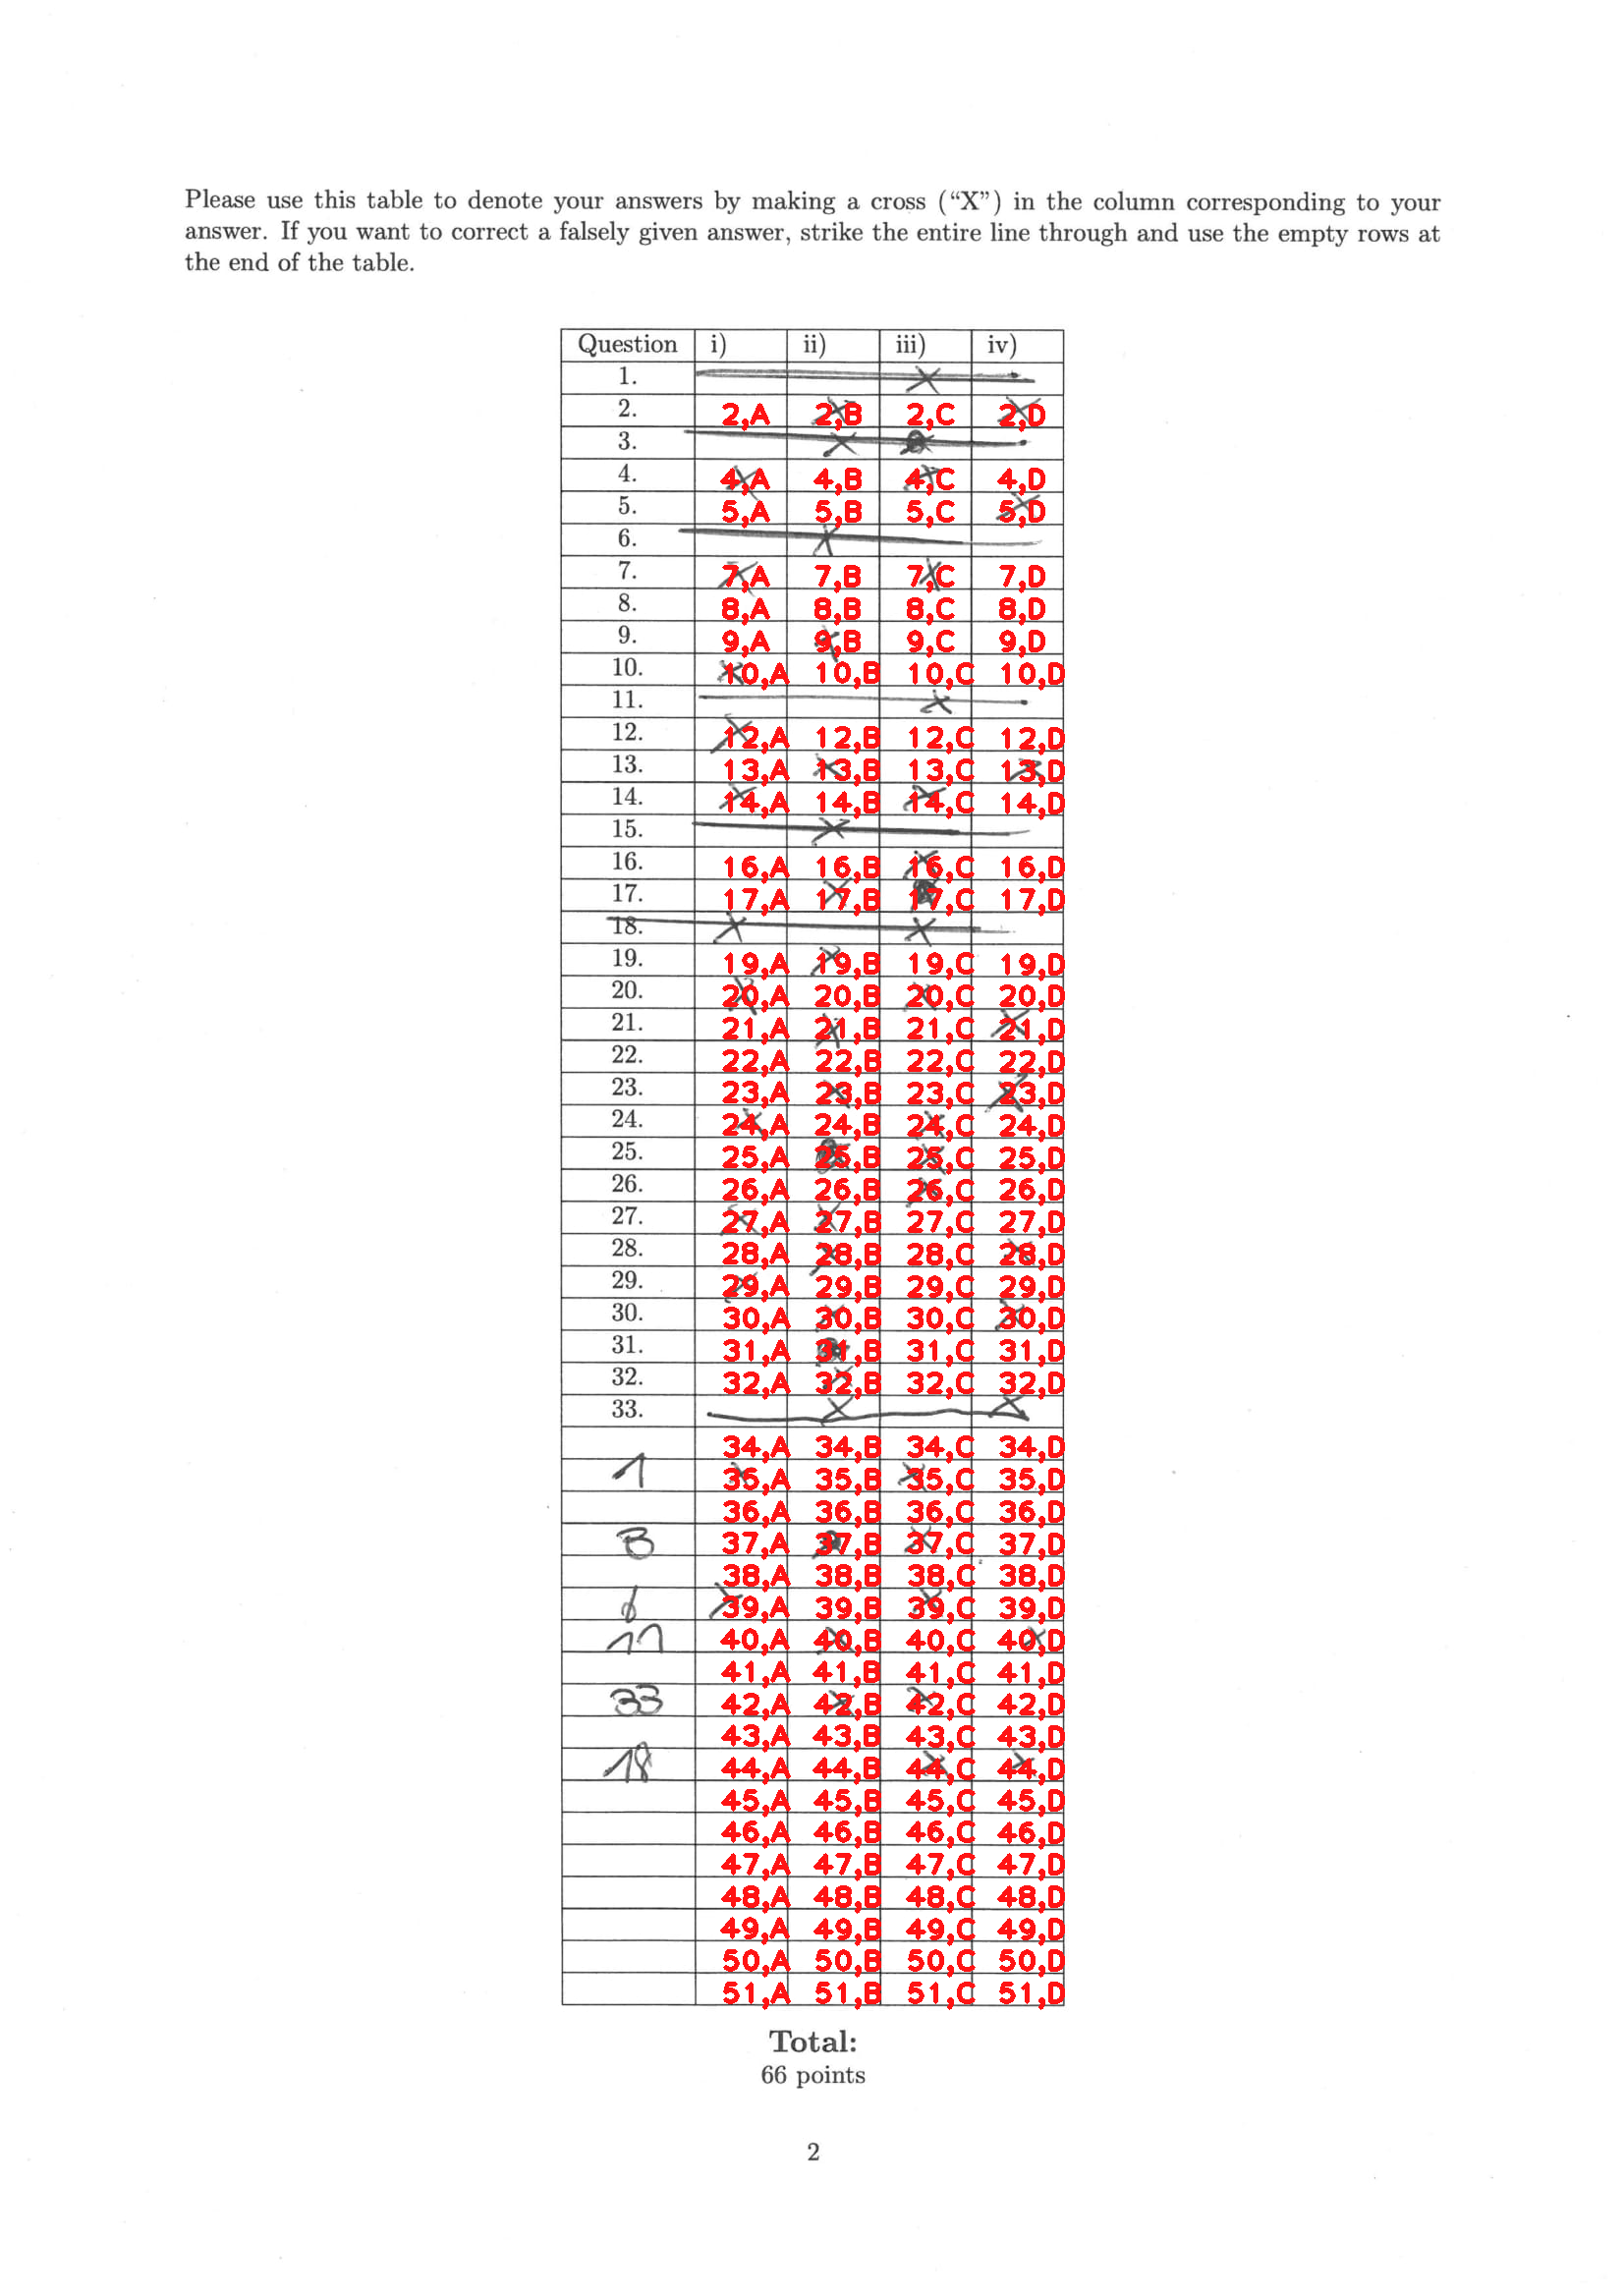
\includegraphics[width=\columnwidth]{Latex/imgs/celldetection.png}
  \caption{calculated locations of cells}
  \label{fig:locations of cells}
 \end{figure}



\subsection{Crosses and self-corrected answers detection}
As know to all, a typical cross consists of two components, and each of them can be regard as a line segment, which inspires us using line detection algorithms such as Hough line transform for this job. Although hough transform has been widely used not only in line detection but also in other curve or shape detection, it has one big drawback. For each nonzero pixel in the image the parameters for the existing curve and redundant ones are both accumulated during the voting procedure, which not only result in large storage requirement but also takes lot of computation and if it was applied to each cell within the table, the runtime for detecting the cells in the whole table will be too long. Thus, in our project we used a probabilistic variant to the classical Hough transform, which have been introduced in \ref{sec:PHT}. It doesn't take all the points into consideration, instead take a only a random subset of points, which is sufficient for line detection but also potentially detect less lines compared to classical Hough Transform. Since this algorithm has been integrated in Opencv library, it is convenient for us to use it directly. This algorithm will be applied to every cell in the table except for the lines that have be crossed out. So that if there is content in a cell, we can get a list of endpoints of the detected lines. \\
As each component of the cross have totally different slope: one must have a positive slope and another has a negative slope accordingly, we can classify the detected lines of into two groups according to their slopes. Then we will each time take one line from one group and another line from another group and calculate the intersection of these two lines. By applying this strategy to all possible combination of lines, we can get a bunch of intersections. Theoretically those intersections are supposed to gather together. Figure \ref{fig: Example_cells_cross} shows the resulting lines marked with purple and intersections marked with red of the a couple of cells that contains cross. It clear to see that those intersections are uniformly distributed and are gathered together which looks like a singe point.\\
In our cases, we not only required to detect the crosses but also need to distinguish the self-corrected answers from the crosses. Typically the self-corrected answers looks like a normal cross but cover with a mass of randomly scratched curves. Similarly, we can apply the probabilistic Hough transform to the cells that contains self-corrected answers and use the same strategy to acquire the intersections of the lines. Figure \ref{fig: Example_cells_self_corrected_answers} gives the results of apply our proposed strategy to a couple of example cells that have self-corrected answers inside. It evident that there are two different result could arise. One is that the lines that the OpenCV function \textit{HoughLinesP()} only have positive or negative slope, e.g. the cell in the first and fourth row and of course there are none intersection that can be found. Another type of results is that the intersection is not uniformly distributed despite these detected lines still can be split into two groups.\\
In order to determine whether the the points have the normal distribution. We will calculated the the covariance matrix based on the coordinates of the intersections. The calculation for the covariance matrix of the two-dimensional variables can be expressed as:
\begin{equation*}
    C = 
    \begin{bmatrix}
    cov(X_1,X_1)&cov(X_1,X_2)\\
    cov(X_2,X_1)&cov(X_2,X_2)
    \end{bmatrix}
\end{equation*}
where $X_1$,$X_2$ refer to scalar random variables. In our cases, they individually represent x-coordinate and y-coordinate. Moreover, we manually set two thresholds T1, T2. If one of $cov(X_1,X_1)$,$cov(X_2,X_2)$ exceeds T1 or $cov(X_1,X_2)$ is bigger than T2, it can be determined that the content in that cell is self-corrected answers, otherwise it is supposed to be regarded as cross.\\
In \ref{appdendix} the algorithm \ref{alg:cross_self_corrected_answers_detection} for detecting the Cross and self-corrected answers is appended, which summarizes all the strategies mentioned in this section.





% \IncMargin{1em}
% \begin{algorithm}
% \SetKwData{Left}{left}\SetKwData{This}{this}\SetKwData{Up}{up}
% \SetKwFunction{Union}{Union}\SetKwFunction{FindCompress}{FindCompress}
% \SetKwInOut{Input}{input}\SetKwInOut{Output}{output}
% \Input{A bitmap $Im$ of size $w\times l$}
% \Output{A partition of the bitmap}
% \BlankLine
% \emph{special treatment of the first line}\;
% \For{$i\leftarrow 2$ \KwTo $l$}{
%   \emph{special treatment of the first element of line $i$}\;
%   \For{$j\leftarrow 2$ \KwTo $w$}{\label{forins}
%     \Left$\leftarrow$ \FindCompress{$Im[i,j-1]$}\;
%     \Up$\leftarrow$ \FindCompress{$Im[i-1,]$}\;
%     \This$\leftarrow$ \FindCompress{$Im[i,j]$}\;
%     \If(\tcp*[h]{O(\Left,\This)==1}){\Left compatible with \This}{\label{lt}
%       \lIf{\Left $<$ \This}{\Union{\Left,\This}}
%       \lElse{\Union{\This,\Left}}
%     }
%     \If(\tcp*[f]{O(\Up,\This)==1}){\Up compatible with \This}{\label{ut}
%       \lIf{\Up $<$ \This}{\Union{\Up,\This}}
%       \tcp{\This is put under \Up to keep tree as flat as possible}\label{cmt}
%       \lElse{\Union{\This,\Up}}\tcp*[h]{\This linked to \Up}\label{lelse}
% } }
%   \lForEach{element $e$ of the line $i$}{\FindCompress{p}}
% }
% \caption{disjoint decomposition}\label{algo_disjdecomp}
% \end{algorithm}\DecMargin{1em}




\begin{figure}[!h]
  \centering
  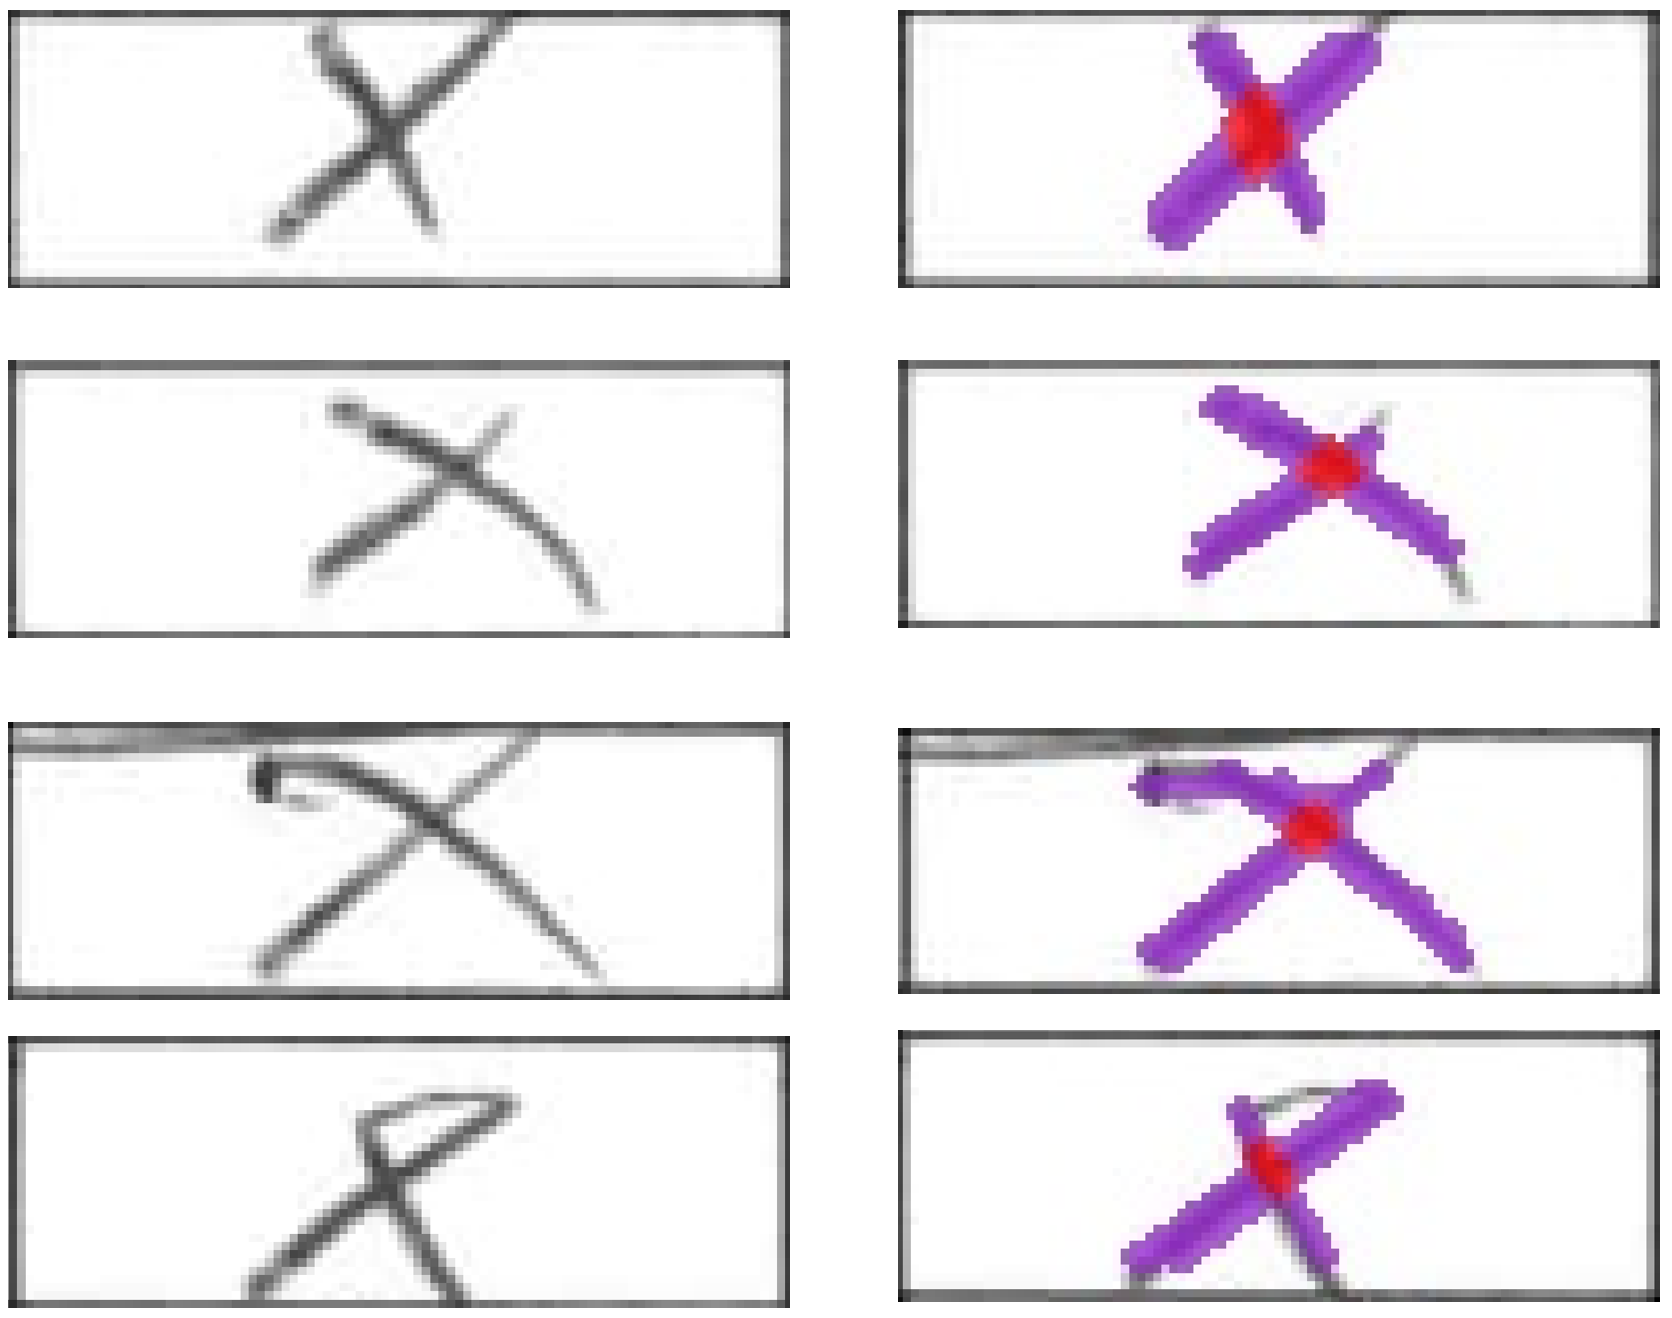
\includegraphics[width=\columnwidth]{Latex/imgs/Crosses_examples.png}
  \caption{Example cells containing cross. The figures on the right-hand side are the corresponding detected lines (marked with purple) and intersections(marked with red) of those lines.}
  \label{fig: Example_cells_cross}
 \end{figure}
\begin{figure}[!h]
  \centering
  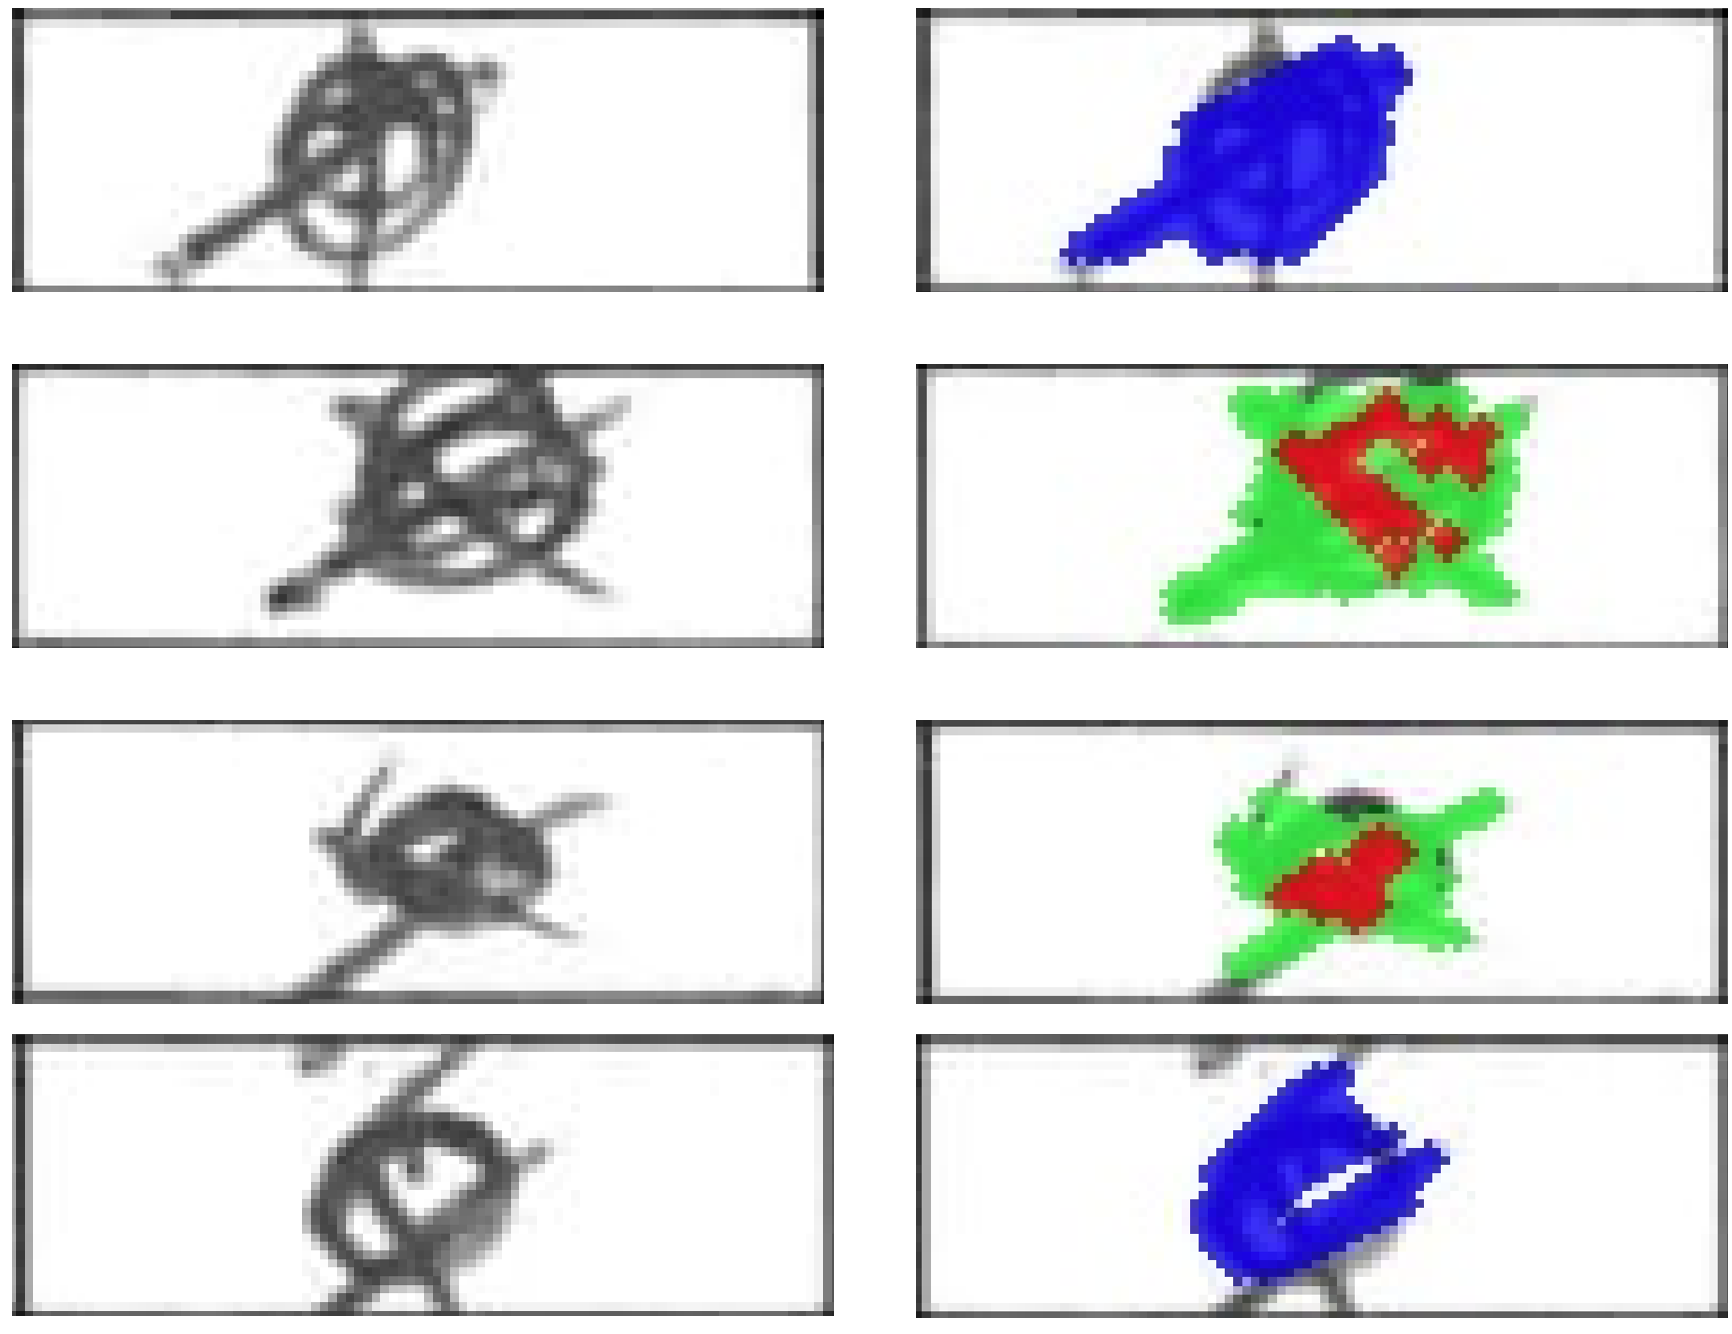
\includegraphics[width=\columnwidth]{Latex/imgs/self_corrected_ansers_example.png}
  \caption{Example cells containing self-corrected answers. The figures on the right-hand side are the corresponding detected lines (marked with blue if all the lines only have positive or negative slope or marked with green if a subset of the  lines have positive slope a others have negative slope) and intersections(marked with red) of those lines.}
  \label{fig: Example_cells_self_corrected_answers}
 \end{figure}

\subsection{GUI}
In order to handle the cases that the crosses might be erroneously detected, and the student may modify their answers by crossing out lines and write a new line down below. The human intervention will be needed to deal with these cases. Therefore, we implemented the graphic user interface with the help of OpenCV library to achieve the objective to edit the answer sheet. The interactive system is made up of 2 modes: Normal mode and Edit mode.\\
In normal mode, users can choose a cell which the cross in it was not detected by the program and change its status as there exists actually a cross in the cell by a single left click.
\begin{figure}[!h]
  \centering
  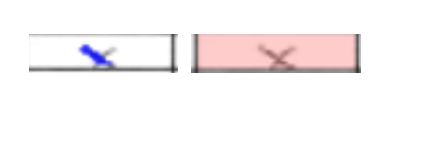
\includegraphics[width=0.8\columnwidth]{Latex/imgs/gui_1.PNG}
  \caption{Example of human intervention, image on the left represents this cross is erroneously detected because only the lines with negative slope  is detected, right side is to force this cell as a crossed cell after human intervention}
  \label{fig: gui_1}
 \end{figure}
 Moreover, if something is erroneously detected as a cross, it needs to be deleted. By single right click we can wipe out the marks in the cell
 \begin{figure}[!h]
  \centering
  
\includegraphics[width=0.8\columnwidth]{Latex/imgs/gui_2.PNG}
  \caption{Example of human intervention, image on the left represents this cell is determined as a crossed cell because lines with positive and negative slopes are detected, image on the right side is to force this cell as a not crossed cell}
  \label{fig: gui_2}
 \end{figure}
In edit mode, users can map the crossed out lines with the new lines down below manually. Firstly, users need to press 'e' to get into the edit mode, then click the task number in the added line down below, after that, click the crossed out lines which the student have crossed out so that these two lines are mapped together. Users can quit the edit mode by simply pressing 'e' again.
 \begin{figure}[!h]
  \centering
  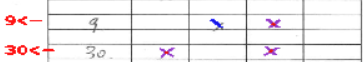
\includegraphics[width=0.8\columnwidth]{Latex/imgs/gui_3.PNG}
  \caption{mapped the hand-written lines with the crossed out lines above manually}
  \label{fig: gui_3}
 \end{figure}
 \subsection{Grading system}
 In last section we introduce a simple GUI which is intended for human intervention. After the mistakes in the generated result are successfully corrected, a two-dimensional array that has the shape of $Nx4$ are supposed to created, where N represents the number of question. In this array the value in the position that corresponds to marked option of a question will be set to True and If there is none cross witin the cell or the check mark is crossed out, then the value is supposed to be set to False. Simiarly the standard answer should also be represented as a two-dimensional array that has the same shape and is created at the same way. The algorithm used for grading the answer sheet are shown in algorithm \ref{alg:Sheet Grading algorithm}.\\
Figure \ref{fig:eventual_result} depicts a example grading result that our implement too eventually generated without human intervention, Where almost all the check marks and self-corrected answers have been detected and the scores of each question and sum of all are shown.


\section{\uppercase{Evaluation}}
In this section we will introduce the performance of our implemented tool on the our dataset. The whole data set composes of 17 answer sheets in total. On each answer sheet the check marks, the lines for crossing rows out and even the self-corrected answers are created with various form or shape to increase the diversity of writing styles and consequently improve the generalization ability of our proposed approach. Due to the manually crafted features and limited size of data set, the evaluation will be performed on the whole data set directly.\\
As stated previously, the abnormal cases contains two specific cases. One is the rows of the table on the answer sheet that could be crossed out by a couple of lines. We have showed in previous section that those rows can be perfectly detected. Thereby, it won't be discussed and evaluated here again. For the convenience the abnormal cases in this section specifically refer to as the second case, the self-corrected answers, which are initially crosses but totally overlapped with casually drafted curves for correcting. A non-blank cell is supposed to be classified either as cross or as abnormal cases.\\ 

\begin{figure}[!h]
  %\vspace{-0.2cm}
  \centering
  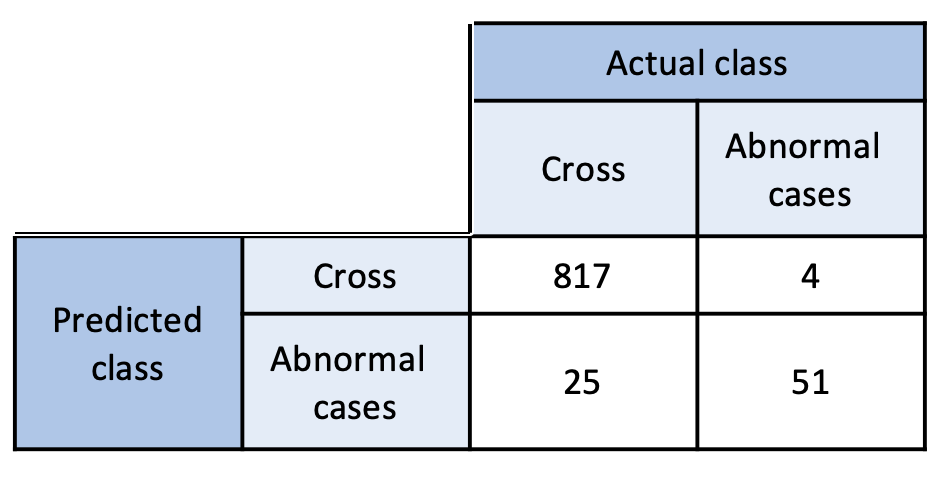
\includegraphics[width=\columnwidth]{Latex/imgs/confusion_matix.png}
  \caption{confusion matrix on our data set}
  \label{fig:confusion_matrix}
 \end{figure}
To visualize the performance of our approach,  a specialized table layout called "Confusion matrix" is utilized, which is widely used in supervised machine learning. the confusion matrix based on our whole dataset are shown in \ref{fig:confusion_matrix}. There are in total 842 crosses existing in our dataset and most of them can be corrected detected expect that 25 crosses are miss-classified as abnormal cases. The number of abnormal cases are much fewer in contrast but accordingly only 4 of them are improperly classified. The figure \ref{fig:class_accuracy} depict the accuracy of detecting crosses and abnormal cases. As you can see the accuracy rate of detecting cross is about $0.970$ while the accuracy rate of abnormal cases detection is a little bit lower but also reaches $0.927$.\\
 \begin{figure}[!h]
  %\vspace{-0.2cm}
  \centering
  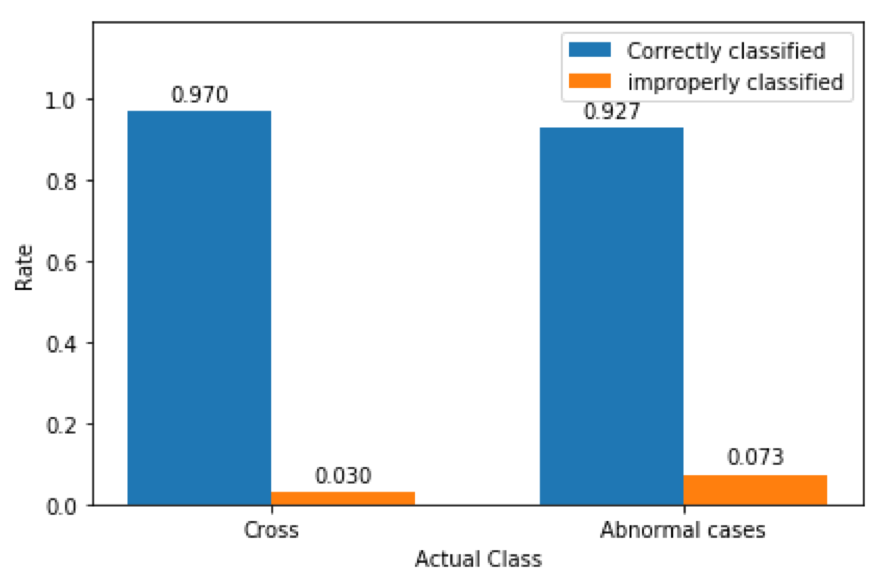
\includegraphics[width=\columnwidth]{Latex/imgs/Bar_figure.png}
  \caption{Overall classification accuracy}
  \label{fig:class_accuracy}
 \end{figure}
Beside the overall performance, we are also concern about the performances on individual answer sheet. Thus, Four example sheet will taken from the dataset, in which the best case and worst case are included. Figure \ref{fig:class_accuracy} shows the confusion matrices of them. The matrix of best case indicates that both the cross and abnormal cases can be perfectly detected. In most cases, there are always 1 or 2 crosses could be falsely detected and in our worst case 6 crosses are not correctly classified.\\
Figure \ref{fig:worst case} shows four example miss-classified crosses on the worst case sheet. The reason why they are not correctly detected is that the probabilistic Hough line function only returned a couple of lines of the one component of the cross. As a result, non-intersection can be found and those crosses will be treated as abnormal cases based on our strategy. In order to  get rid of the problem lot of methods to have been tried, such as decrease the minimum length of the lines that Hough line transform can detect. Although it may get the performance on that sheet better, the overall performance can be even worse. Maybe introducing more features can eventually work with those problems and can achieve more accurate results.\\
 \begin{figure}[!h]
  %\vspace{-0.2cm}
  \centering
  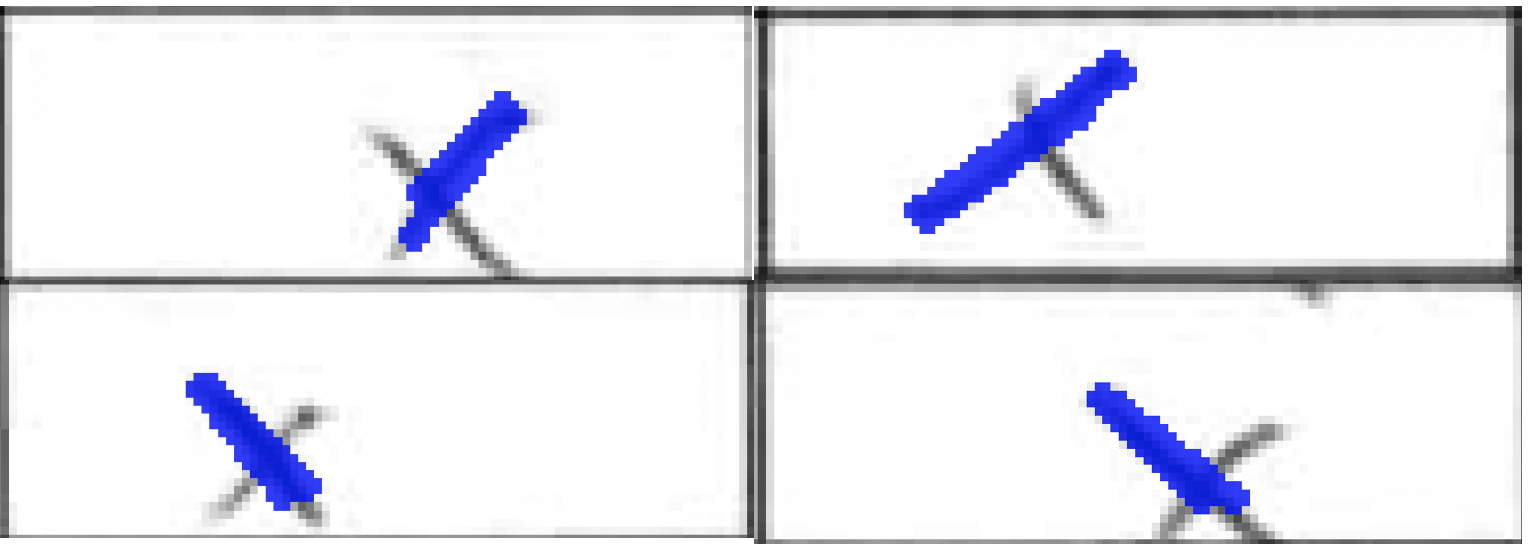
\includegraphics[width=\columnwidth]{Latex/imgs/notdetected.png}
  \caption{Example miss-classified crosses on the worst case sheet.}
  \label{fig:worst case}
 \end{figure}



 

  \begin{figure}[!h]
  %\vspace{-0.2cm}
  \centering
  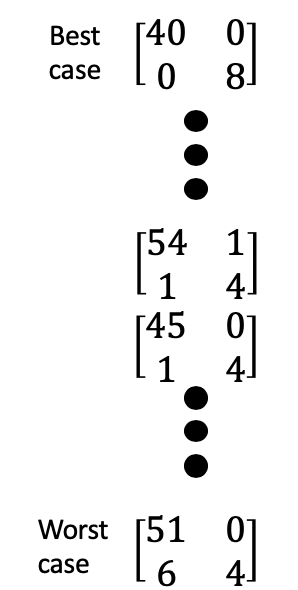
\includegraphics[width=0.4\columnwidth]{Latex/imgs/4matrix.png}
  \caption{Confusion matrices of example answer sheet in our data set including best and worst case.}
  \label{fig:class_accuracy}
 \end{figure}



\section{\uppercase{Conclusions  and future work}}
\label{sec:conclusion}
\subsection{Conclusion}
In this project, we implemented a viable tool to automatically grading the answer sheet of exam. This tool can detected the crossed out rows with hundred percentage accuracy and flag those rows for human intervention. The accuracy of detecting the check marks in the table of the answer sheet can reach 0.97 on our dataset while the accuracy of detecting the abnormal cases is a little bit lower but still achieves 0.927. Moreover, a specify interactive system is designed which give the users the chances to correct the generated results. Beside that we also implement a function which take the previously generated data such as detected crosses for grading the result. Those results will be wrote on the image so that user can check the result later. 
\subsection{future work}
\begin{figure}[!h]
  \centering
  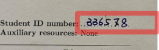
\includegraphics[width=0.8\columnwidth]{Latex/imgs/digit.PNG}
  \caption{An example of student ID number}
  \label{fig: ID}
 \end{figure}
It would be extremely convinient if the program can recognize the student ID number automatically. The hand-written digit recognition is not a difficult problem if the digits are isolated. i.e. digits are independent between each other. From MNIST dataset, there are 60,000 examples for training and 10,000 examples for testing, all the digits are size-normalized and centered. However, in reality, it is very possible that the digits of the hand-written ID are independent, which means, the student IDs are connected numerical strings. In the research of Ribas et al. \cite{ribas2013handwritten}, they compared different digits segmentation algorithms. Fujisawa et al. \cite{fujisawa1992segmentation} proposed a recognition-based algorithm that detect all the connected components of the images and classifies them into isolated digits or string of digits. The principle of classification is set a threshold for the horizontal length of the connected components. In order to handling touching digits, the algorithm splits the contour into upper and lower contours and use another threshold of vertical width to approximate the potential segmentation points. For example for the numerical strings like "0-0", "8-8", the third threshold is set to isolate the loops of left and right according to the distance between them. The approach proposed by Shi and Govindaraju \cite{shi1997segmentation} is based on the observation that touching points and ligatures between two
digits reveal that the chaincode contour makes significant right turns at each point of touching. The methods assumes that the touching pair is free of slant. The final segmentation point is approximated using vertical histogram and a set of heuristics. Moreover, Chen and Wang \cite{chen2000segmentation} presented their ideas of combining background and foreground analysis to segment handwritten numeral strings. Fisrtly, the foreground and background regions on image of connected numeral string are thinned, and
the feature points on foreground and background skeletons
are extracted. Therefore, some possible segmentation paths can be constructed and ligatures are removed. Finally, the parameters of the geometric properties of every possible segmentation path are approximated. These parameters are calculated
by a mixture of Gaussian probability functions to decide on
the best segmentation path or rejection of a path 





\vfill
\bibliographystyle{apalike}
{\small
\bibliography{grader_bib}}

\newpage
\onecolumn
\section*{\uppercase{Appendix}}
\label{appdendix}
\begin{figure}[!h]
  %\vspace{-0.2cm}
  \centering
  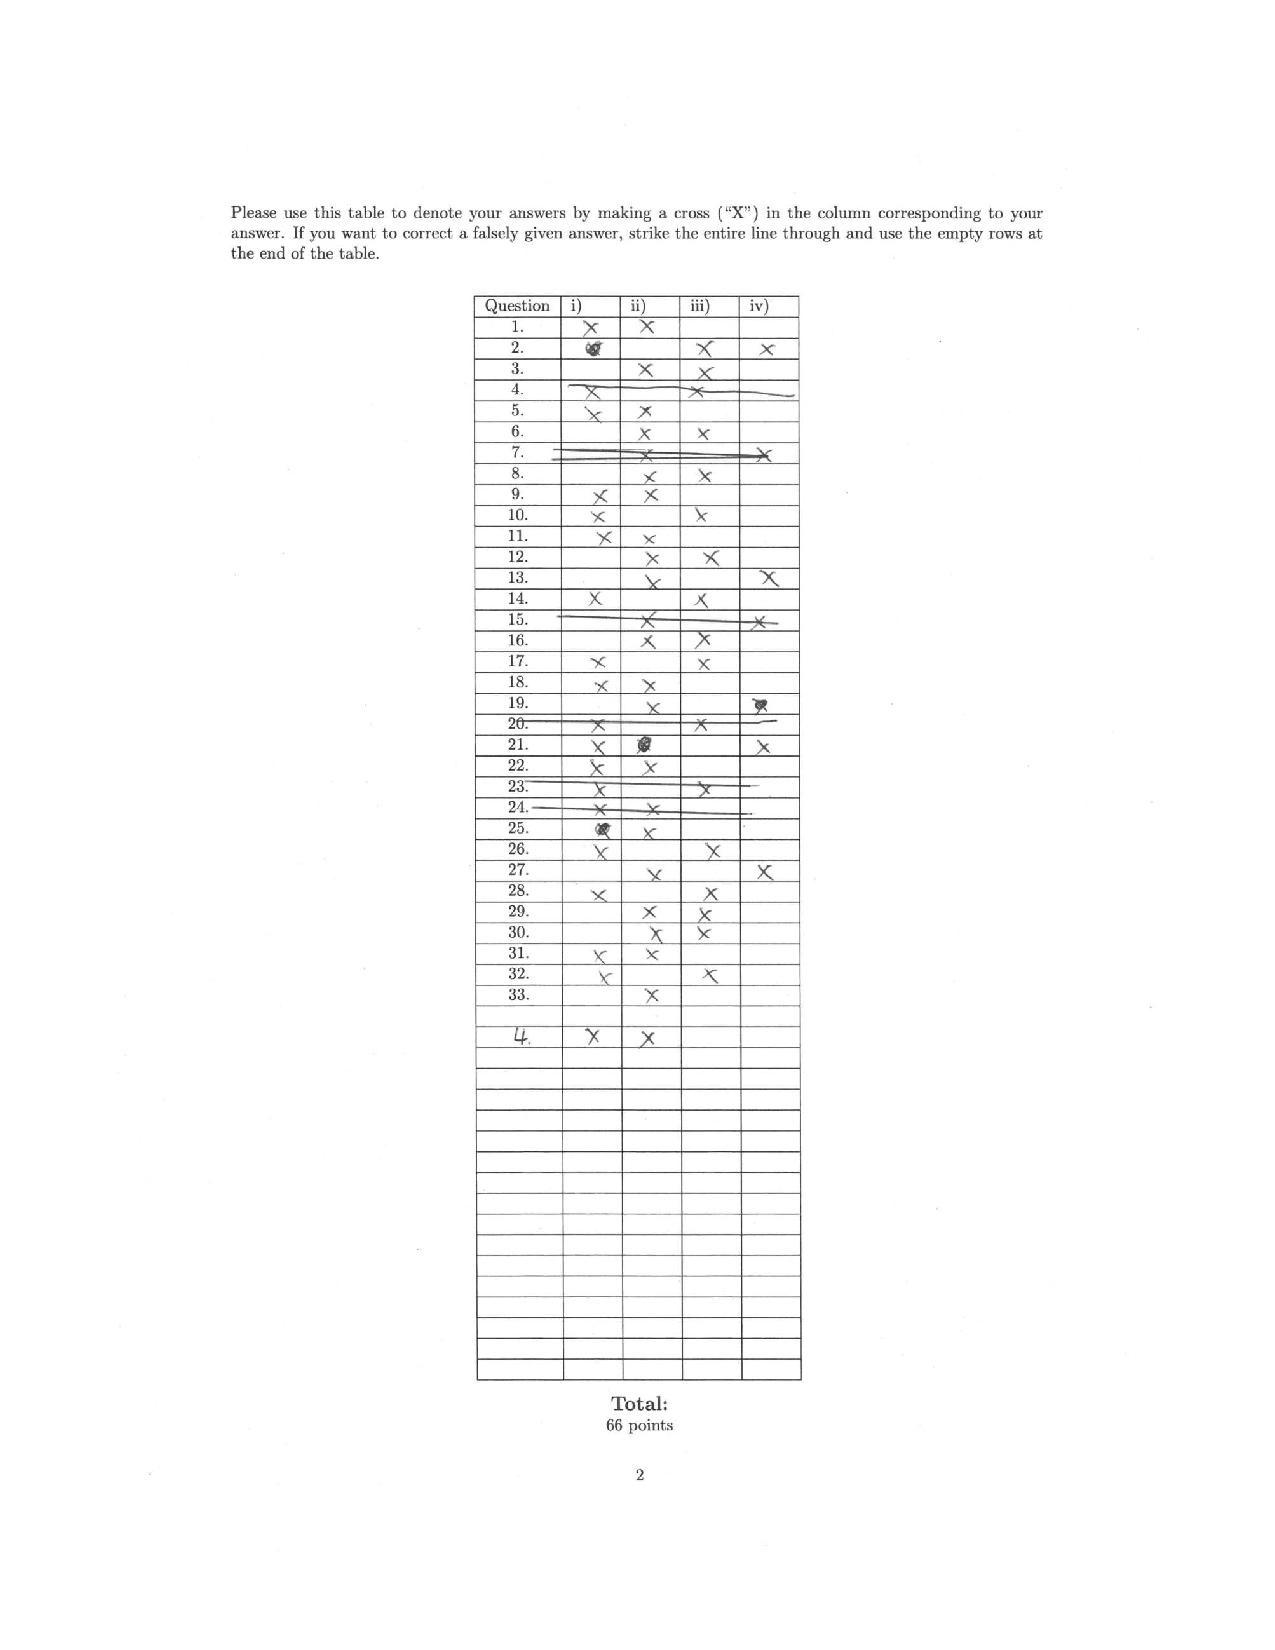
\includegraphics[width=\columnwidth]{Latex/imgs/example_answer_sheet.pdf}
  \caption{Example answer sheet taken from our created date set}
  \label{fig:example_answer_sheet}
 \end{figure}
 
 \begin{figure}[!h]
  %\vspace{-0.2cm}
  \centering
  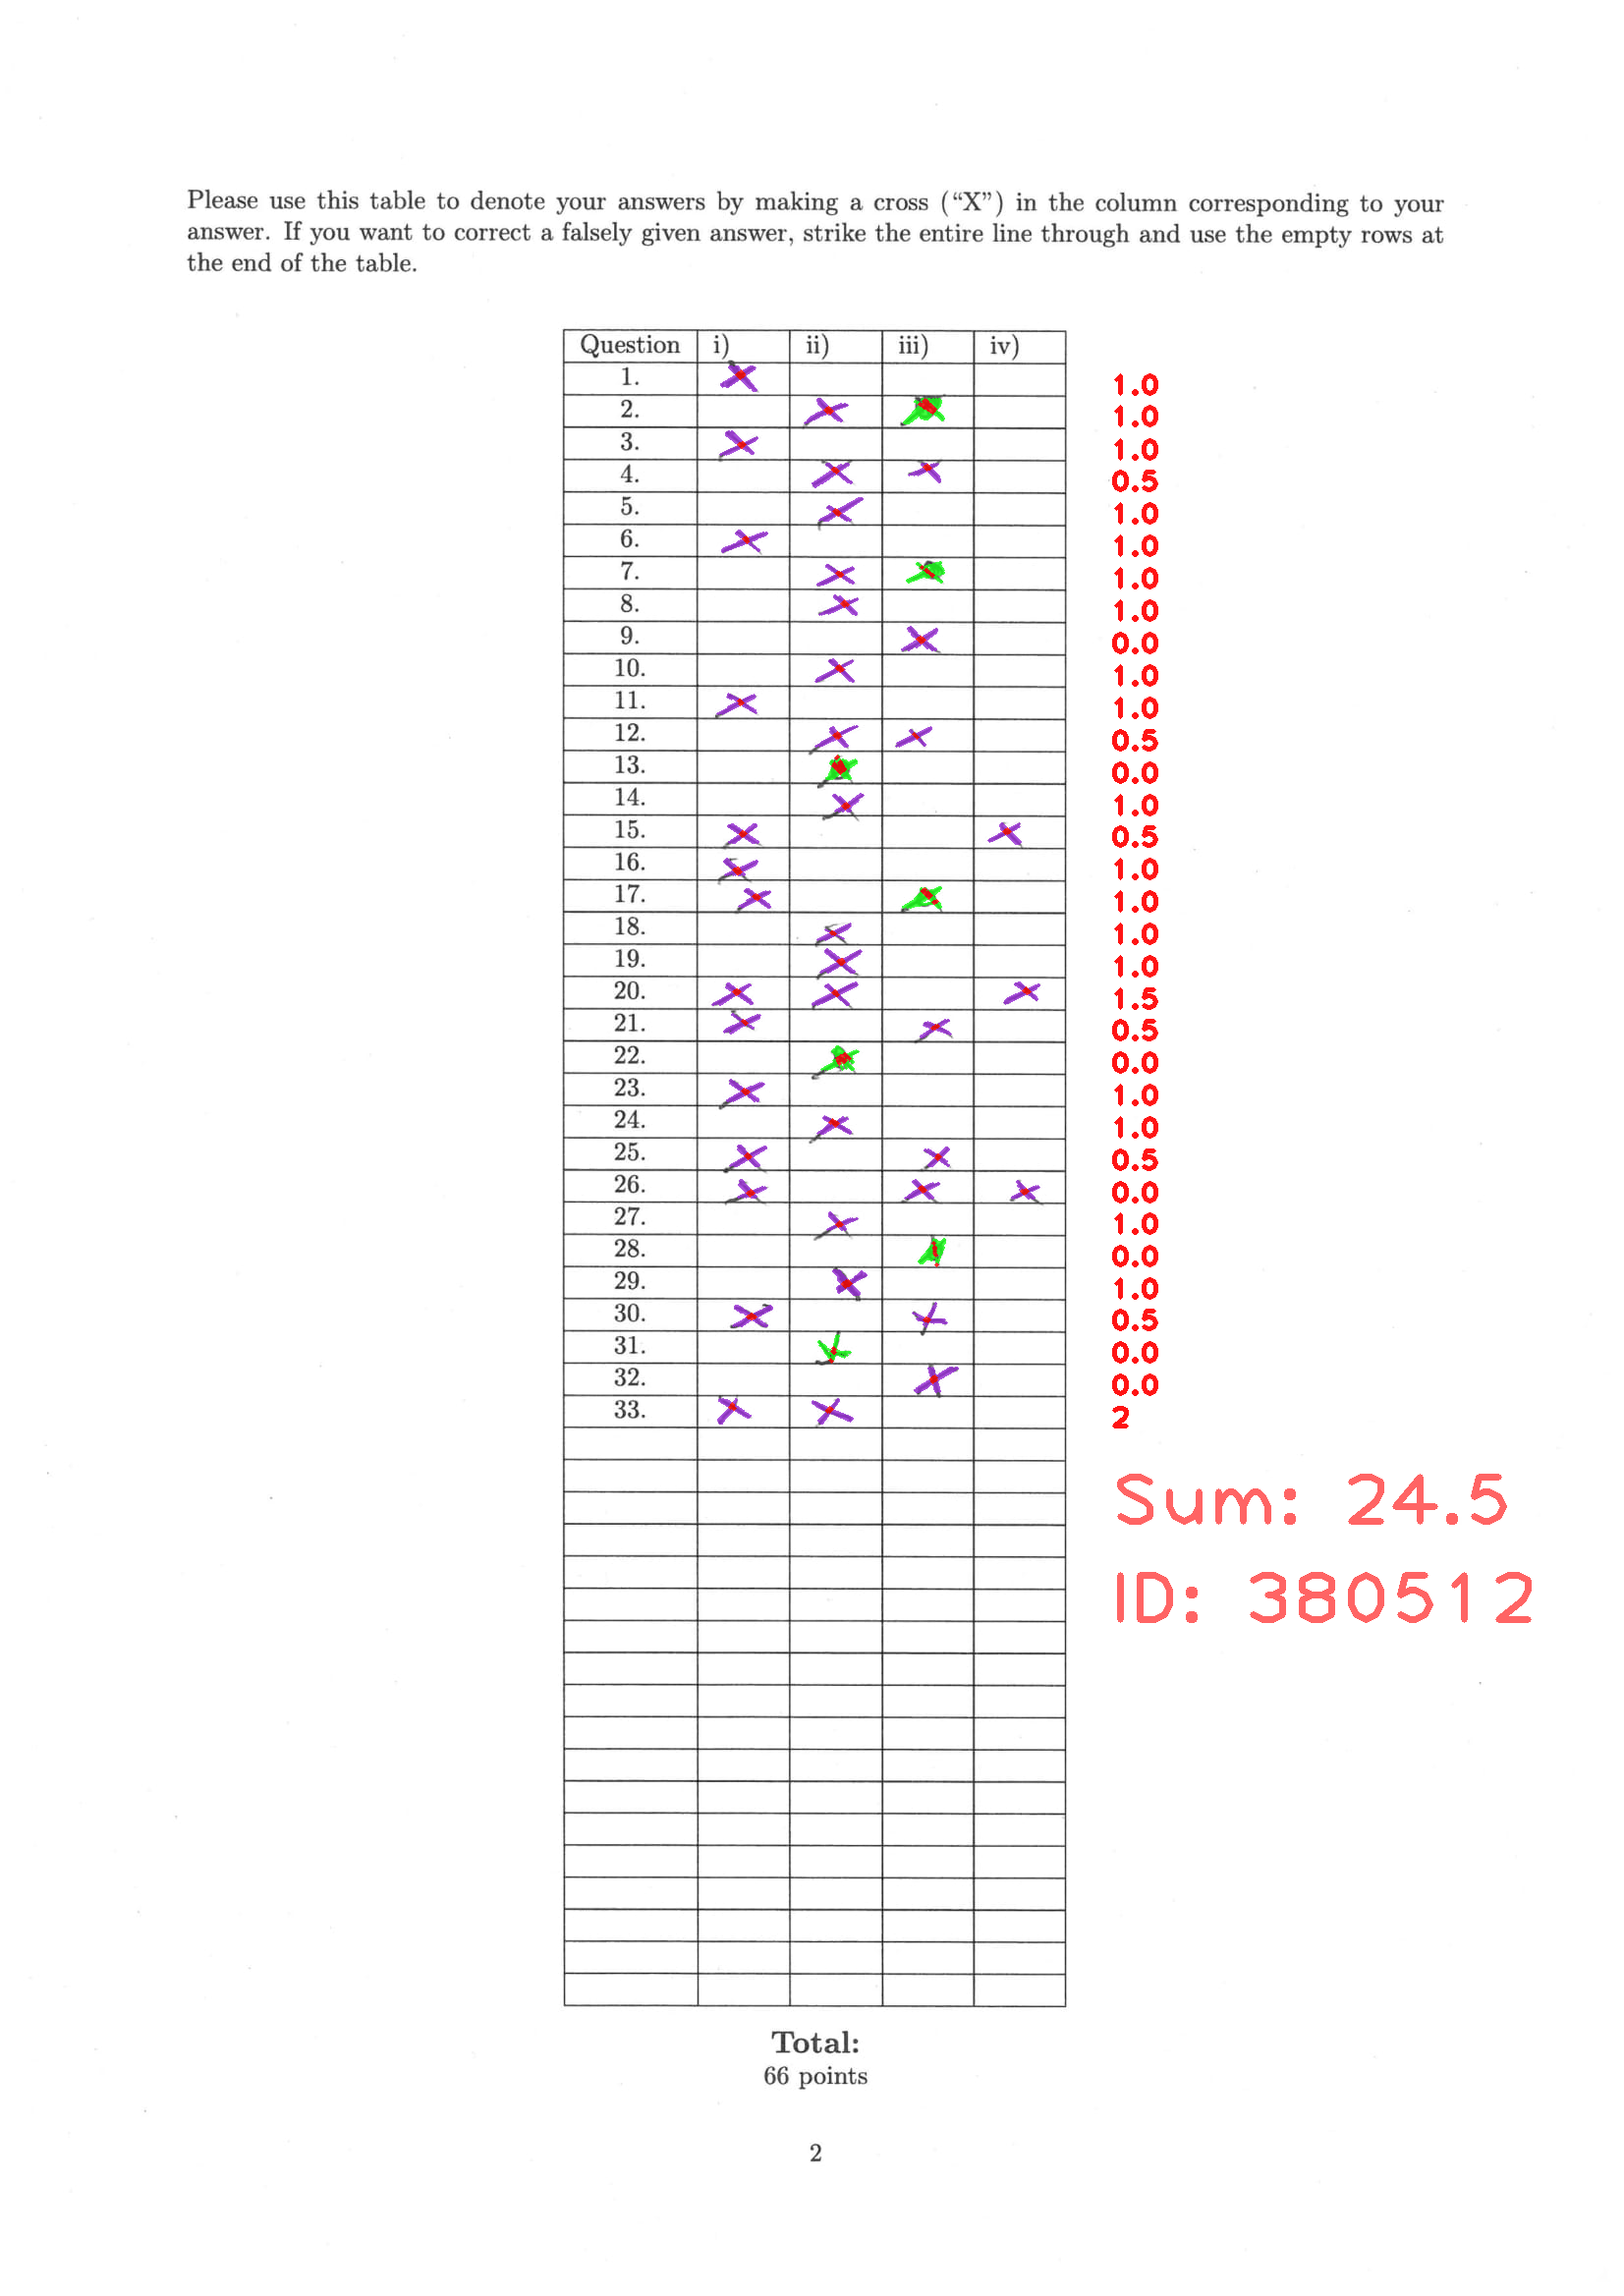
\includegraphics[width=\columnwidth]{Latex/imgs/380512.png}
  \caption{Example grading result that our implement tool eventually generate without human intervention here , where the scores of each question and sum of them are all depicted in the figure.}
  \label{fig:eventual_result}
 \end{figure}
 
 
 
 
 \IncMargin{1em}
\begin{algorithm}
\SetKwInOut{Input}{Input}\SetKwInOut{Outputa}{Output1}\SetKwInOut{Outputb}{Output2}
\SetKwData{Table}{Table}
\SetKwData{llIsCross}{llIsCross}
\SetKwData{llIsSelfCorrectedAnswer}{llIsSelfCorrectedAnswer}
\SetKwData{Row}{Row}
\SetKwData{None}{None}
\SetKwData{Cell}{Cell}
\SetKwData{isCross}{isCross}
\SetKwData{isSelfCorrectedAnswer}{isSelfCorrectedAnswer}
\SetKwData{Intersections}{Intersections}
\SetKwFunction{SplitLines}{SplitLines}
\SetKwFunction{HoughLinesP}{HoughLinesP}
\SetKwFunction{CalculateIntersections}{CalculateIntersections}
\SetKwFunction{AnalyzePointsDistribution}{AnalyzePointsDistribution}
\SetKw{in}{in}
\Input{ \textbf{\textit{Table}}:  a list of rows, if the row is crossed out, None will be saved, otherwise row is supposed to be a list of cells }
\Outputa{\textbf{\textit{llIsCross}}: a list of list of Boolean Value isCross}
\Outputb{\textbf{\textit{llIsSelfCorrectedAnswer}}: a list of list of Boolean Value isSelfCorrectedAnswer}
\BlankLine
\For{\Row \in \Table}{
    \tcp*[h]{Row is not crossed out}\;
    \If{\Row is not \None}{
    lIsCross = list()\;
    lIsSelfCorrectedAnswer = list()\;
    \For{\Cell \in \Row and \Cell is not first one}{
        \tcp{skip the first column}\ 
        \If{Cell is not first component in \Row}{
            \isCross = False\; 
            \isSelfCorrectedAnswer = False\;
            lines = \HoughLinesP{\Cell}\;
            LineGroups = \SplitLines{lines}\;
            \tcp*[h]{All lines belong to one line group as the slopes of them are all positive or negative}\;
            \uIf{len(LinesGroups) ==1}{isSelfCorrectedAnswer = True}
            \Else{
            \Intersections = \CalculateIntersections{GroupsLines}\;
            ArePointsConcentrated = \AnalyzePointsDistribution{\Intersections}\;
            \lIf{ArePointsConcentrated is True}{ isCross = True }
            \lElse{isSelfCorrectedAnswer = True}
            }
            lIsCross.append(isCross)\;
            lIsSelfCorrectedAnswer.append(isSelfCorrectedAnswer)
        }
    llIsCross.append(lIsCross)\;
    llIsSelfCorrectedAnswer.append(lIsSelfCorrectedAnswer)\;
    }
    }
}
\caption{Crosses and self-corrected Answers detection Algorithm}
\label{alg:cross_self_corrected_answers_detection}
\end{algorithm}
\DecMargin{1em}

 \IncMargin{1em}
 \begin{algorithm}
  \SetKw{in}{in}
  \SetKwInOut{Inputa}{Input1}
  \SetKwInOut{Inputb}{Input2}
  \SetKwInOut{Inputc}{Input3}
  \SetKwInOut{Output}{Output}
  \SetKwData{Question}{Question}
  \SetKwData{Questions}{Questions}
  \Inputa{ \textbf{\textit{ArrayAnswersStudent}}:  the two-dimensional array that stores the answers of current answer sheet, shape: N x 4 }
  \Inputb{ \textbf{\textit{ArrayAnswersstandard}}: standard answers, shape: N x 4 }
  \Inputc{ \textbf{\textit{ArrayPointsQuestions}}: the points of each check mark in corresponding question, shape N }
  \Output{\textbf{\textit{Scores}}}
  \BlankLine
  PointsTotal = 0
  \For{\Question \in \Questions}{
         \tcp*[h]{Shape: 1 x 4 }\;
        CurrentQuestionAnswerStudent = ArrayAnswersStudent(\Question)\;
        \tcp*[h]{Shape: 1 x 4 }\;
        CurrentQuestionAnswerStandard = ArrayAnswersstandard(\Question)\;
        \tcp*[h]{Shape: 1 }\;
        CurrentQuestionPoints = ArrayPointsQuestions(\Question)\;
        \tcp*[h]{Apply element-wise logical-and to these two array, Shape 1 x 4}\;
        CorrectAnswers = LogicalAnd(CurrentQuestionAnswerStudent,CurrentQuestionAnswerStandard)\;
        \tcp*[h]{Shape: 1 x 4 }\;
        WrongAnswers = LogicalXOR(CurrentQuestionAnswerStudent,CorrectAnswers)\;
        \tcp*[h]{calculate the points to current question and make sure it is not less than 0}\;
        PointsCurrentQuestion = MAX((SUM(CorrectAnswers)-SUM(WrongAnswers)/2)*CurrentQuestionPoints,0)\;
        PointsTotal = PointsTotal+PointsCurrentQuestion\;
  }
\caption{Sheet Grading algorithm}
\label{alg:Sheet Grading algorithm}
\end{algorithm}
 \DecMargin{1em}
 
 
 
 



\vfill
\end{document}